\documentclass[border=8pt]{standalone}
\usepackage{amsmath,amssymb}
\usepackage{tikz}
\usetikzlibrary{arrows.meta,decorations.markings,shadings,calc,positioning,fit,backgrounds}
\definecolor{flux}{RGB}{238,118,22}
\definecolor{ink}{RGB}{32,38,52}
\tikzset{lab/.style={font=\footnotesize,text=ink,align=left,fill=white,fill opacity=0.88,text opacity=1,inner sep=1.5pt,rounded corners=1pt},
         lead/.style={draw=ink!50,line width=0.45pt},
         ptitle/.style={font=\bfseries\small,text=ink,anchor=west},
         box/.style={draw=ink!22,rounded corners=4pt,line width=0.6pt}}
\begin{document}
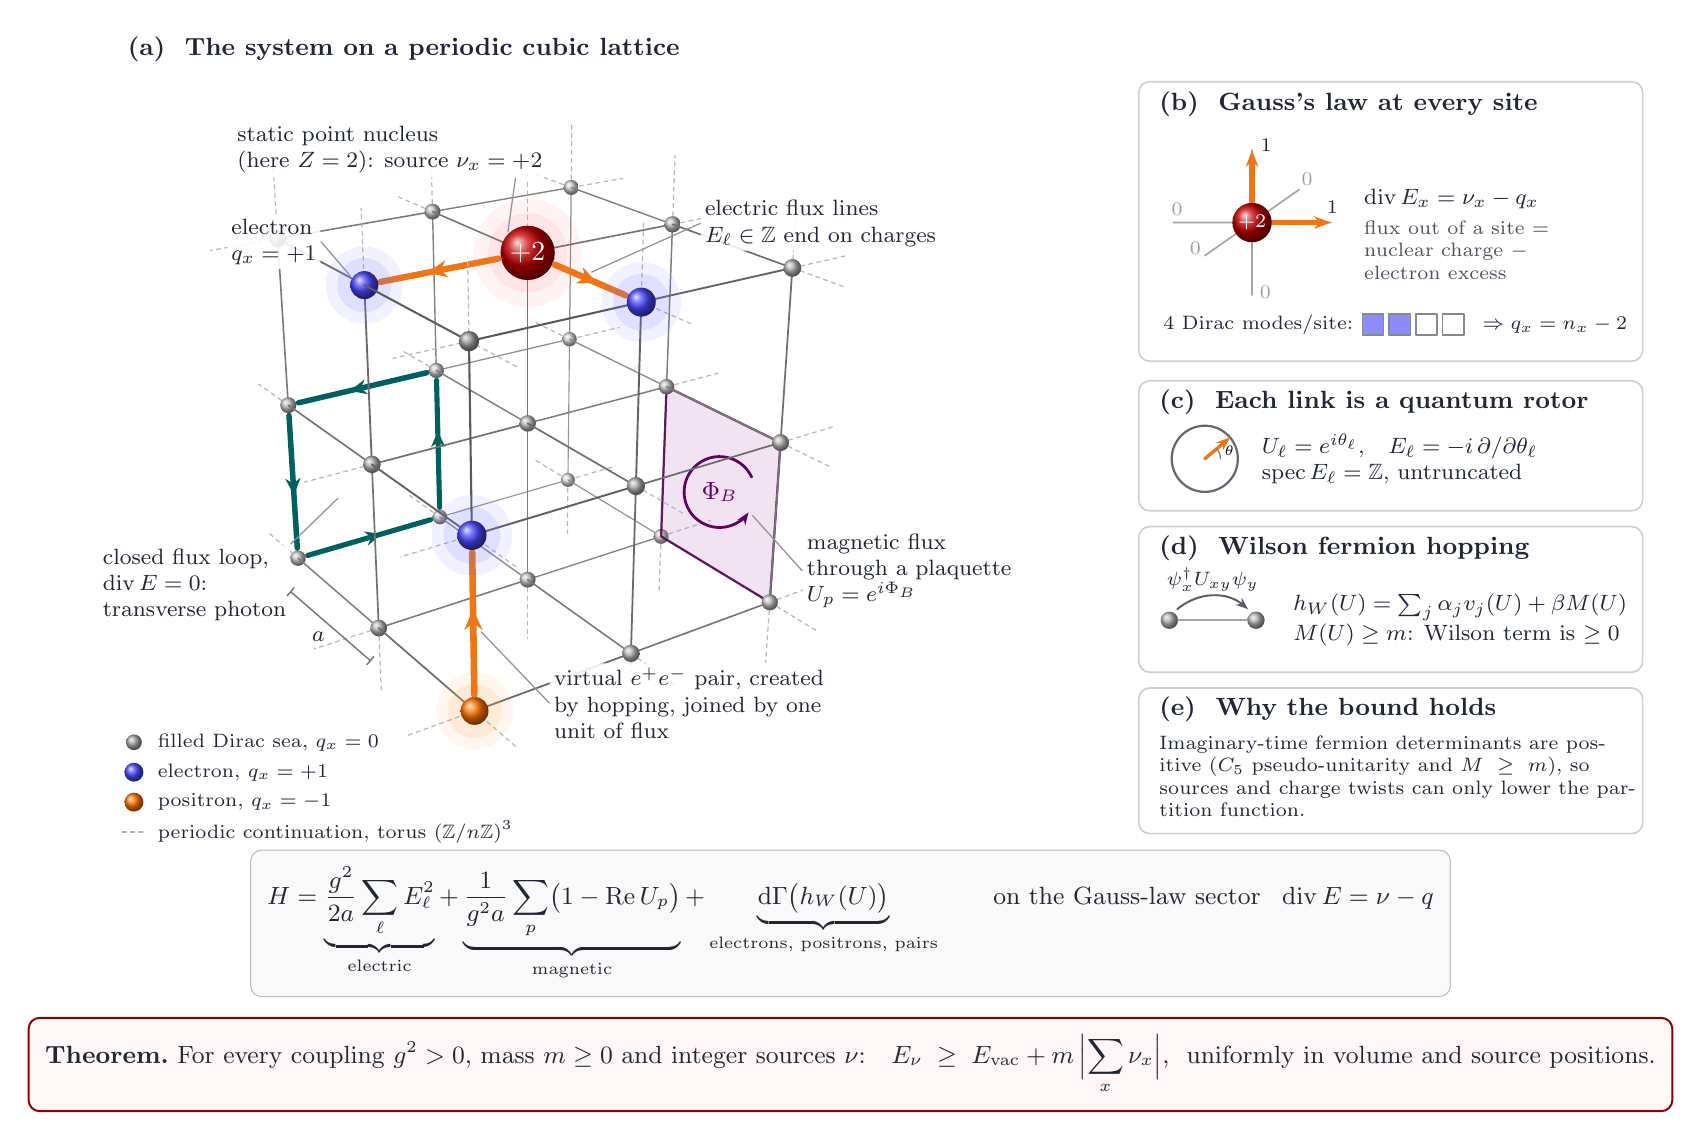
\begin{tikzpicture}[line cap=round,line join=round]
%=========================== (a) ===========================
\begin{scope}
\coordinate (N) at (0.000,2.165);
\coordinate (e1) at (-2.074,1.756);
\coordinate (e2) at (1.443,1.540);
\coordinate (P) at (-0.674,-3.652);
\coordinate (Q) at (-0.708,-1.422);
\coordinate (loop) at (-2.058,-0.500);
\coordinate (mag) at (2.437,-0.872);
\coordinate (a0) at (-2.916,-1.712);
\coordinate (a1) at (-1.891,-2.599);
\coordinate (top) at (0.553,2.996);
\coordinate (c000) at (-2.916,-1.712);
\coordinate (c200) at (-0.674,-3.652);
\coordinate (c022) at (0.553,2.996);
\coordinate (c220) at (3.075,-2.272);

\draw[line width=0.45pt,draw=black!28,dash pattern=on 1.5pt off 1.5pt] (0.512,-0.718) -- (0.085,-0.459);
\draw[line width=0.45pt,draw=black!28,dash pattern=on 1.5pt off 1.5pt] (0.512,-0.718) -- (1.120,-0.541);
\draw[line width=0.45pt,draw=black!28,dash pattern=on 1.5pt off 1.5pt] (0.512,-0.718) -- (0.505,-1.396);
\draw[line width=0.40pt,draw=black!42!white] (0.512,-0.718) -- (0.532,1.069);
\draw[line width=0.41pt,draw=black!42!white] (-1.115,-1.190) -- (0.512,-0.718);
\shade[ball color=black!16] (0.512,-0.718) circle (0.089);
\draw[line width=0.45pt,draw=black!28,dash pattern=on 1.5pt off 1.5pt] (0.532,1.069) -- (0.088,1.286);
\draw[line width=0.45pt,draw=black!28,dash pattern=on 1.5pt off 1.5pt] (0.532,1.069) -- (1.162,1.217);
\draw[line width=0.42pt,draw=black!43!white] (0.512,-0.718) -- (1.695,-1.435);
\draw[line width=0.45pt,draw=black!28,dash pattern=on 1.5pt off 1.5pt] (-1.115,-1.190) -- (-1.516,-0.904);
\draw[line width=0.45pt,draw=black!45!white] (0.532,1.069) -- (0.553,2.996);
\draw[line width=0.45pt,draw=black!45!white] (-1.160,0.672) -- (0.532,1.069);
\shade[ball color=black!19] (0.532,1.069) circle (0.092);
\draw[line width=0.45pt,draw=black!28,dash pattern=on 1.5pt off 1.5pt] (1.695,-1.435) -- (2.324,-1.231);
\draw[line width=0.45pt,draw=black!28,dash pattern=on 1.5pt off 1.5pt] (1.695,-1.435) -- (1.668,-2.154);
\draw[line width=0.45pt,draw=black!28,dash pattern=on 1.5pt off 1.5pt] (0.553,2.996) -- (0.092,3.164);
\draw[line width=0.45pt,draw=black!28,dash pattern=on 1.5pt off 1.5pt] (0.553,2.996) -- (1.207,3.110);
\draw[line width=0.45pt,draw=black!28,dash pattern=on 1.5pt off 1.5pt] (0.553,2.996) -- (0.562,3.811);
\draw[line width=0.47pt,draw=black!46!white] (0.532,1.069) -- (1.764,0.465);
\shade[ball color=black!19] (-1.115,-1.190) circle (0.093);
\draw[line width=0.45pt,draw=black!28,dash pattern=on 1.5pt off 1.5pt] (-1.160,0.672) -- (-1.575,0.912);
\draw[line width=0.48pt,draw=black!47!white] (-1.115,-1.190) -- (0.000,-1.985);
\draw[line width=0.49pt,draw=black!48!white] (1.695,-1.435) -- (1.764,0.465);
\draw[line width=1.85pt,draw=teal!75!black,postaction={decorate},decoration={markings,mark=at position 0.6 with {\arrow{Stealth[length=5.7pt,width=5.1pt]}}}] (-1.118,-1.067) -- (-1.157,0.545);
\draw[line width=0.45pt,draw=black!28,dash pattern=on 1.5pt off 1.5pt] (-2.916,-1.712) -- (-3.282,-1.396);
\draw[line width=0.50pt,draw=black!48!white] (0.000,-1.985) -- (1.695,-1.435);
\draw[line width=1.86pt,draw=teal!75!black,postaction={decorate},decoration={markings,mark=at position 0.6 with {\arrow{Stealth[length=5.8pt,width=5.2pt]}}}] (-2.793,-1.677) -- (-1.233,-1.224);
\draw[line width=0.50pt,draw=black!49!white] (-1.208,2.689) -- (0.553,2.996);
\shade[ball color=black!21] (1.695,-1.435) circle (0.095);
\shade[ball color=black!21] (0.553,2.996) circle (0.096);
\draw[line width=0.51pt,draw=black!49!white] (-1.160,0.672) -- (-1.208,2.689);
\draw[line width=0.45pt,draw=black!28,dash pattern=on 1.5pt off 1.5pt] (1.764,0.465) -- (2.418,0.637);
\draw[line width=0.51pt,draw=black!49!white] (1.695,-1.435) -- (3.075,-2.272);
\draw[line width=0.52pt,draw=black!50!white] (0.553,2.996) -- (1.840,2.528);
\shade[ball color=black!22] (-1.160,0.672) circle (0.097);
\draw[line width=0.45pt,draw=black!28,dash pattern=on 1.5pt off 1.5pt] (0.000,-1.985) -- (0.000,-2.733);
\draw[line width=0.45pt,draw=black!28,dash pattern=on 1.5pt off 1.5pt] (-1.208,2.689) -- (-1.638,2.875);
\draw[line width=0.45pt,draw=black!28,dash pattern=on 1.5pt off 1.5pt] (-1.208,2.689) -- (-1.229,3.543);
\draw[line width=0.53pt,draw=black!50!white] (-1.160,0.672) -- (0.000,0.000);
\fill[violet!50,opacity=0.22] (1.695,-1.435) -- (3.075,-2.272) -- (3.212,-0.244) -- (1.764,0.465) -- cycle; \draw[violet!65!black,line width=0.8pt,opacity=0.85] (1.695,-1.435) -- (3.075,-2.272) -- (3.212,-0.244) -- (1.764,0.465) -- cycle;
\shade[ball color=black!23] (-2.916,-1.712) circle (0.098);
\draw[line width=0.54pt,draw=black!51!white] (1.764,0.465) -- (1.840,2.528);
\draw[line width=0.45pt,draw=black!28,dash pattern=on 1.5pt off 1.5pt] (-3.040,0.231) -- (-3.417,0.498);
\draw[line width=0.54pt,draw=black!51!white] (-2.916,-1.712) -- (-1.891,-2.599);
\draw[line width=0.54pt,draw=black!51!white] (0.000,0.000) -- (1.764,0.465);
\draw[line width=1.97pt,draw=teal!75!black,postaction={decorate},decoration={markings,mark=at position 0.6 with {\arrow{Stealth[length=6.1pt,width=5.4pt]}}}] (-1.283,0.643) -- (-2.911,0.261);
\draw[violet!75!black,line width=1pt,-{Stealth[length=4.5pt]}] ($ (2.437,-0.872) + (25:0.45) $) arc[start angle=25,end angle=325,radius=0.45]; \node[violet!75!black,font=\small] at (2.437,-0.872) {$\Phi_B$};
\shade[ball color=black!24] (1.764,0.465) circle (0.099);
\draw[line width=0.55pt,draw=black!52!white] (0.000,-1.985) -- (0.000,0.000);
\draw[line width=1.98pt,draw=teal!75!black,postaction={decorate},decoration={markings,mark=at position 0.6 with {\arrow{Stealth[length=6.1pt,width=5.5pt]}}}] (-3.031,0.099) -- (-2.925,-1.585);
\draw[line width=0.45pt,draw=black!28,dash pattern=on 1.5pt off 1.5pt] (3.075,-2.272) -- (3.694,-2.648);
\draw[line width=0.45pt,draw=black!28,dash pattern=on 1.5pt off 1.5pt] (3.075,-2.272) -- (3.726,-2.033);
\draw[line width=0.45pt,draw=black!28,dash pattern=on 1.5pt off 1.5pt] (3.075,-2.272) -- (3.023,-3.036);
\draw[line width=0.45pt,draw=black!28,dash pattern=on 1.5pt off 1.5pt] (1.840,2.528) -- (2.519,2.662);
\draw[line width=0.45pt,draw=black!28,dash pattern=on 1.5pt off 1.5pt] (1.840,2.528) -- (1.872,3.403);
\draw[line width=0.56pt,draw=black!52!white] (-1.891,-2.599) -- (0.000,-1.985);
\draw[line width=0.56pt,draw=black!52!white] (1.764,0.465) -- (3.212,-0.244);
\draw[line width=0.56pt,draw=black!53!white] (-3.174,2.345) -- (-1.208,2.689);
\shade[ball color=black!24] (0.000,-1.985) circle (0.101);
\shade[ball color=black!25] (-1.208,2.689) circle (0.101);
\draw[line width=0.57pt,draw=black!53!white] (-3.040,0.231) -- (-3.174,2.345);
\draw[line width=0.57pt,draw=black!53!white] (0.000,-1.985) -- (1.312,-2.921);
\draw[line width=0.58pt,draw=black!54!white] (-1.208,2.689) -- (0.000,2.165);
\shade[ball color=black!25] (-3.040,0.231) circle (0.102);
\draw[line width=0.58pt,draw=black!54!white] (3.075,-2.272) -- (3.212,-0.244);
\draw[line width=0.45pt,draw=black!28,dash pattern=on 1.5pt off 1.5pt] (-1.891,-2.599) -- (-2.711,-2.864);
\draw[line width=0.45pt,draw=black!28,dash pattern=on 1.5pt off 1.5pt] (-1.891,-2.599) -- (-1.859,-3.379);
\draw[line width=0.45pt,draw=black!28,dash pattern=on 1.5pt off 1.5pt] (-3.174,2.345) -- (-3.562,2.554);
\draw[line width=0.45pt,draw=black!28,dash pattern=on 1.5pt off 1.5pt] (-3.174,2.345) -- (-4.025,2.197);
\draw[line width=0.45pt,draw=black!28,dash pattern=on 1.5pt off 1.5pt] (-3.174,2.345) -- (-3.231,3.244);
\draw[line width=0.59pt,draw=black!54!white] (1.312,-2.921) -- (3.075,-2.272);
\draw[line width=0.59pt,draw=black!55!white] (-3.040,0.231) -- (-1.978,-0.521);
\draw[line width=0.59pt,draw=black!55!white] (0.000,2.165) -- (1.840,2.528);
\shade[ball color=black!26] (3.075,-2.272) circle (0.103);
\shade[ball color=black!26] (1.840,2.528) circle (0.104);
\draw[line width=0.60pt,draw=black!55!white] (0.000,0.000) -- (0.000,2.165);
\draw[line width=0.45pt,draw=black!28,dash pattern=on 1.5pt off 1.5pt] (3.212,-0.244) -- (3.865,-0.563);
\draw[line width=0.45pt,draw=black!28,dash pattern=on 1.5pt off 1.5pt] (3.212,-0.244) -- (3.888,-0.041);
\draw[line width=0.61pt,draw=black!56!white] (-1.978,-0.521) -- (0.000,0.000);
\draw[line width=0.61pt,draw=black!56!white] (1.840,2.528) -- (3.362,1.974);
\shade[ball color=black!27] (0.000,0.000) circle (0.105);
\draw[line width=0.61pt,draw=black!56!white] (-1.891,-2.599) -- (-1.978,-0.521);
\draw[line width=0.45pt,draw=black!28,dash pattern=on 1.5pt off 1.5pt] (1.312,-2.921) -- (1.905,-3.343);
\draw[line width=0.45pt,draw=black!28,dash pattern=on 1.5pt off 1.5pt] (1.312,-2.921) -- (1.289,-3.718);
\draw[line width=0.45pt,draw=black!28,dash pattern=on 1.5pt off 1.5pt] (0.000,2.165) -- (0.000,3.087);
\draw[line width=0.62pt,draw=black!57!white] (0.000,0.000) -- (1.375,-0.796);
\shade[ball color=black!28] (-1.891,-2.599) circle (0.106);
\shade[ball color=black!28] (-3.174,2.345) circle (0.107);
\draw[line width=0.63pt,draw=black!57!white] (3.212,-0.244) -- (3.362,1.974);
\draw[line width=0.45pt,draw=black!28,dash pattern=on 1.5pt off 1.5pt] (-1.978,-0.521) -- (-2.839,-0.748);
\draw[line width=0.63pt,draw=black!57!white] (-1.891,-2.599) -- (-0.674,-3.652);
\draw[line width=0.63pt,draw=black!57!white] (1.375,-0.796) -- (3.212,-0.244);
\draw[line width=0.64pt,draw=black!58!white] (-3.174,2.345) -- (-2.074,1.756);
\shade[ball color=black!29] (3.212,-0.244) circle (0.108);
\draw[line width=0.64pt,draw=black!58!white] (1.312,-2.921) -- (1.375,-0.796);
\draw[line width=0.45pt,draw=black!28,dash pattern=on 1.5pt off 1.5pt] (3.362,1.974) -- (4.052,1.723);
\draw[line width=0.45pt,draw=black!28,dash pattern=on 1.5pt off 1.5pt] (3.362,1.974) -- (4.065,2.133);
\draw[line width=0.45pt,draw=black!28,dash pattern=on 1.5pt off 1.5pt] (3.362,1.974) -- (3.426,2.920);
\draw[line width=0.65pt,draw=black!58!white] (-0.674,-3.652) -- (1.312,-2.921);
\shade[ball color=black!29] (1.312,-2.921) circle (0.110);
\fill[red!60,opacity=0.08] (0.000,2.165) circle (0.690); \fill[red!60,opacity=0.10] (0.000,2.165) circle (0.502); \shade[ball color=red!78!black] (0.000,2.165) circle (0.345); \node[white,font=\bfseries] at (0.000,2.165) {$+2$};
\draw[line width=0.66pt,draw=black!59!white] (-1.978,-0.521) -- (-2.074,1.756);
\draw[line width=0.45pt,draw=black!28,dash pattern=on 1.5pt off 1.5pt] (1.375,-0.796) -- (1.999,-1.158);
\shade[ball color=black!30] (-1.978,-0.521) circle (0.111);
\draw[line width=0.45pt,draw=black!28,dash pattern=on 1.5pt off 1.5pt] (-0.674,-3.652) -- (-0.120,-4.130);
\draw[line width=0.45pt,draw=black!28,dash pattern=on 1.5pt off 1.5pt] (-0.674,-3.652) -- (-1.540,-3.970);
\draw[line width=0.45pt,draw=black!28,dash pattern=on 1.5pt off 1.5pt] (-2.074,1.756) -- (-2.115,2.730);
\draw[line width=0.68pt,draw=black!61!white] (-1.978,-0.521) -- (-0.708,-1.422);
\draw[line width=0.68pt,draw=black!61!white] (1.443,1.540) -- (3.362,1.974);
\draw[line width=2.27pt,draw=flux,postaction={decorate},decoration={markings,mark=at position 0.6 with {\arrow{Stealth[length=7.0pt,width=6.2pt]}}}] (-0.368,2.093) -- (-1.870,1.796);
\shade[ball color=black!31] (3.362,1.974) circle (0.113);
\draw[line width=0.69pt,draw=black!61!white] (1.375,-0.796) -- (1.443,1.540);
\draw[line width=0.70pt,draw=black!62!white] (-0.708,-1.422) -- (1.375,-0.796);
\draw[line width=2.30pt,draw=flux,postaction={decorate},decoration={markings,mark=at position 0.6 with {\arrow{Stealth[length=7.1pt,width=6.3pt]}}}] (0.344,2.016) -- (1.247,1.625);
\shade[ball color=black!32] (1.375,-0.796) circle (0.115);
\draw[line width=0.45pt,draw=black!28,dash pattern=on 1.5pt off 1.5pt] (1.443,1.540) -- (2.102,1.254);
\draw[line width=0.45pt,draw=black!28,dash pattern=on 1.5pt off 1.5pt] (1.443,1.540) -- (1.473,2.541);
\fill[orange!70,opacity=0.10] (-0.674,-3.652) circle (0.488); \fill[orange!70,opacity=0.15] (-0.674,-3.652) circle (0.344); \shade[ball color=orange!90!red] (-0.674,-3.652) circle (0.177);
\fill[blue!55,opacity=0.10] (-2.074,1.756) circle (0.489); \fill[blue!55,opacity=0.14] (-2.074,1.756) circle (0.345); \shade[ball color=blue!72] (-2.074,1.756) circle (0.178);
\draw[line width=0.45pt,draw=black!28,dash pattern=on 1.5pt off 1.5pt] (-0.708,-1.422) -- (-0.126,-1.835);
\draw[line width=0.45pt,draw=black!28,dash pattern=on 1.5pt off 1.5pt] (-0.708,-1.422) -- (-1.620,-1.697);
\draw[line width=0.73pt,draw=black!64!white] (-2.074,1.756) -- (-0.745,1.044);
\draw[line width=2.38pt,draw=flux,postaction={decorate},decoration={markings,mark=at position 0.6 with {\arrow{Stealth[length=7.4pt,width=6.5pt]}}}] (-0.677,-3.444) -- (-0.704,-1.639);
\draw[line width=0.74pt,draw=black!65!white] (-0.745,1.044) -- (1.443,1.540);
\fill[blue!55,opacity=0.10] (1.443,1.540) circle (0.505); \fill[blue!55,opacity=0.14] (1.443,1.540) circle (0.356); \shade[ball color=blue!72] (1.443,1.540) circle (0.184);
\draw[line width=0.75pt,draw=black!65!white] (-0.708,-1.422) -- (-0.745,1.044);
\fill[blue!55,opacity=0.10] (-0.708,-1.422) circle (0.513); \fill[blue!55,opacity=0.14] (-0.708,-1.422) circle (0.361); \shade[ball color=blue!72] (-0.708,-1.422) circle (0.186);
\draw[line width=0.45pt,draw=black!28,dash pattern=on 1.5pt off 1.5pt] (-0.745,1.044) -- (-0.133,0.716);
\draw[line width=0.45pt,draw=black!28,dash pattern=on 1.5pt off 1.5pt] (-0.745,1.044) -- (-1.709,0.826);
\draw[line width=0.45pt,draw=black!28,dash pattern=on 1.5pt off 1.5pt] (-0.745,1.044) -- (-0.762,2.106);
\shade[ball color=black!38] (-0.745,1.044) circle (0.129);
\node[lab,anchor=south] (Ln) at ($(N)+(-1.75,0.95)$) {static point nucleus\\ (here $Z=2$): source $\nu_x=+2$};
\draw[lead] ($(Ln.south east)+(-0.4,0)$) -- ($(N)+(-0.25,0.27)$);
\node[lab,anchor=east] (Le) at ($(e1)+(-0.55,0.55)$) {electron\\ $q_x=+1$};
\draw[lead] (Le.east) -- ($(e1)+(-0.18,0.12)$);
\node[lab,anchor=west] (Lf) at ($(e2)+(0.75,1.0)$) {electric flux lines\\ $E_\ell\in\mathbb Z$ end on charges};
\draw[lead] (Lf.west) -- ($(N)!0.55!(e2)+(0.02,0.1)$);
\node[lab,anchor=west] (Lp) at ($(P)+(0.95,0.1)$) {virtual $e^+e^-$ pair, created\\ by hopping, joined by one\\ unit of flux};
\draw[lead] (Lp.west) -- ($(P)!0.45!(Q)+(0.1,0)$);
\node[lab,anchor=east] (Ll) at ($(loop)+(-0.95,-1.55)$) {closed flux loop,\\ $\operatorname{div}E=0$:\\ transverse photon};
\draw[lead] (Ll.north east) -- ($(loop)+(-0.35,-0.45)$);
\node[lab,anchor=west] (Lm) at ($(mag)+(1.05,-1.0)$) {magnetic flux\\ through a plaquette\\ $U_p=e^{i\Phi_B}$};
\draw[lead] (Lm.west) -- ($(mag)+(0.42,-0.3)$);
\draw[ink!65,line width=0.5pt,{Bar[width=4pt]}-{Bar[width=4pt]}] ($(c000)+(-0.1,-0.42)$) -- node[below left=-2pt,font=\footnotesize,text=ink]{$a$} ($(a1)+(-0.1,-0.42)$);
\node[font=\bfseries\small,text=ink,anchor=west] at (-5.2,4.75) {(a)\ \ The system on a periodic cubic lattice};
% legend
\begin{scope}[shift={(-5.0,-4.05)}]
 \shade[ball color=black!35] (0,0) circle (0.1);  \node[font=\scriptsize,text=ink,anchor=west] at (0.18,0) {filled Dirac sea, $q_x=0$};
 \shade[ball color=blue!72] (0,-0.38) circle (0.12); \node[font=\scriptsize,text=ink,anchor=west] at (0.18,-0.38) {electron, $q_x=+1$};
 \shade[ball color=orange!90!red] (0,-0.76) circle (0.12); \node[font=\scriptsize,text=ink,anchor=west] at (0.18,-0.76) {positron, $q_x=-1$};
 \draw[line width=0.45pt,draw=black!30,dash pattern=on 1.5pt off 1.5pt] (-0.15,-1.14)--(0.12,-1.14); \node[font=\scriptsize,text=ink,anchor=west] at (0.18,-1.14) {periodic continuation, torus $(\mathbb Z/n\mathbb Z)^3$};
\end{scope}
\end{scope}
%======================== right column =======================
\begin{scope}[shift={(8.15,0)}]
\node[box,minimum width=6.4cm,minimum height=3.55cm,anchor=north west] (B) at (-0.4,4.35) {};
\node[ptitle] at (-0.25,4.05) {(b)\ \ Gauss's law at every site};
\begin{scope}[shift={(1.05,2.55)}]
 \draw[line width=0.6pt,black!35] (-1.0,0)--(1.0,0) (0,-0.92)--(0,0.92) (-0.6,-0.42)--(0.6,0.42);
 \draw[line width=2pt,flux,-{Stealth[length=6pt]}] (0.27,0)--(1.0,0);
 \draw[line width=2pt,flux,-{Stealth[length=6pt]}] (0,0.27)--(0,0.92);
 \shade[ball color=red!78!black] (0,0) circle (0.25); \node[white,font=\bfseries\scriptsize] at (0,0) {$+2$};
 \node[font=\scriptsize,text=ink] at (1.02,0.2) {$1$}; \node[font=\scriptsize,text=ink] at (0.18,0.98) {$1$};
 \foreach \p in {(-0.95,0.17),(0.17,-0.88),(0.7,0.55),(-0.72,-0.32)} \node[font=\scriptsize,text=ink!45] at \p {$0$};
\end{scope}
\node[font=\footnotesize,text=ink,anchor=west,align=left] at (2.35,2.85) {$\displaystyle\operatorname{div}E_x=\nu_x-q_x$};
\node[font=\scriptsize,text=ink!80,anchor=west,align=left] at (2.35,2.2) {flux out of a site $=$\\ nuclear charge $-$\\ electron excess};
\begin{scope}[shift={(0.0,1.25)}]
 \node[font=\scriptsize,text=ink,anchor=west] at (-0.2,0) {4 Dirac modes/site:};
 \foreach \i/\c in {0/blue!45,1/blue!45,2/white,3/white}{\draw[ink!55,line width=0.5pt,fill=\c] (2.45+0.34*\i,-0.13) rectangle ++(0.27,0.27);}
 \node[font=\scriptsize,text=ink,anchor=west] at (3.85,0) {$\Rightarrow q_x=n_x-2$};
\end{scope}
%-- (c)
\node[box,minimum width=6.4cm,minimum height=1.65cm,anchor=north west] at (-0.4,0.55) {};
\node[ptitle] at (-0.25,0.27) {(c)\ \ Each link is a quantum rotor};
\begin{scope}[shift={(0.45,-0.45)}]
 \draw[ink!70,line width=0.8pt] (0,0) circle (0.42);
 \draw[flux,line width=1.2pt,-{Stealth[length=5pt]}] (0,0) -- (40:0.42);
 \draw[ink!55,line width=0.5pt] (0.2,0) arc[start angle=0,end angle=40,radius=0.2];
 \node[font=\tiny] at (0.31,0.1) {$\theta$};
\end{scope}
\node[font=\footnotesize,text=ink,anchor=west,align=left] at (1.05,-0.45) {$U_\ell=e^{i\theta_\ell}$,\quad $E_\ell=-i\,\partial/\partial\theta_\ell$\\ $\operatorname{spec}E_\ell=\mathbb Z$, untruncated};
%-- (d)
\node[box,minimum width=6.4cm,minimum height=1.85cm,anchor=north west] at (-0.4,-1.3) {};
\node[ptitle] at (-0.25,-1.58) {(d)\ \ Wilson fermion hopping};
\begin{scope}[shift={(0.0,-2.5)}]
 \shade[ball color=black!30] (0,0) circle (0.11); \shade[ball color=black!30] (1.1,0) circle (0.11);
 \draw[black!35,line width=0.6pt] (0.11,0)--(0.99,0);
 \draw[ink!75,line width=0.7pt,-{Stealth[length=4.5pt]}] (0.1,0.14) to[bend left=40] (1.0,0.14);
 \node[font=\scriptsize,text=ink] at (0.55,0.52) {$\psi^\dagger_xU_{xy}\psi_y$};
\end{scope}
\node[font=\footnotesize,text=ink,anchor=west,align=left] at (1.45,-2.5) {$h_W(U)=\sum_j\alpha_j v_j(U)+\beta M(U)$\\ $M(U)\ge m$: Wilson term is $\ge0$};
%-- (e) positivity
\node[box,minimum width=6.4cm,minimum height=1.85cm,anchor=north west] at (-0.4,-3.35) {};
\node[ptitle] at (-0.25,-3.63) {(e)\ \ Why the bound holds};
\node[font=\scriptsize,text=ink,anchor=north west,align=left,text width=6.1cm] at (-0.25,-3.85)
 {Imaginary-time fermion determinants are positive ($C_5$ pseudo-unitarity and $M\ge m$), so sources and charge twists can only lower the partition function.};
\end{scope}
%========================= bottom strip ======================
\begin{scope}[shift={(4.1,-6.35)}]
 \node[draw=ink!30,rounded corners=4pt,fill=black!2.5,inner sep=6pt,font=\small,text=ink] (H) at (0,0)
 {$\displaystyle H=\underbrace{\frac{g^2}{2a}\sum_{\ell}E_\ell^2}_{\text{electric}}
 +\underbrace{\frac{1}{g^2a}\sum_{p}\bigl(1-\operatorname{Re}U_p\bigr)}_{\text{magnetic}}
 +\underbrace{\mathrm d\Gamma\bigl(h_W(U)\bigr)}_{\text{electrons, positrons, pairs}}
 \qquad \text{on the Gauss-law sector }\ \operatorname{div}E=\nu-q$};
 \node[draw=red!55!black,line width=0.7pt,rounded corners=4pt,fill=red!3,inner sep=6pt,font=\small,text=ink,anchor=north] at ($(H.south)+(0,-0.25)$)
 {\textbf{Theorem.}\ For every coupling $g^2>0$, mass $m\ge0$ and integer sources $\nu$:\quad
 $\displaystyle E_\nu\;\ge\;E_{\mathrm{vac}}+m\,\Bigl|\sum_x\nu_x\Bigr|$,\ \ uniformly in volume and source positions.};
\end{scope}
\end{tikzpicture}
\end{document}
